\title{Homework 1 Solutions for Computer Logic and Circuit Design: PHYS306/COSC330}
\author{Dr. Jordan Hanson - Whittier College Dept. of Physics and Astronomy}
\date{\today}
\documentclass[10pt]{article}
\usepackage[a4paper, total={18cm, 27cm}]{geometry}
\usepackage{graphicx}
\begin{document}
\maketitle

\section{1-2: Binary Digits, Logic Levels, and Digital Waveforms}

\begin{enumerate}
\item Exercise 7: a) 0.6 $\mu$s, from 0.2 to 0.8 $\mu$s.  Remeber the convention is 10-90 percent of the amplitude. b) 0.55 $\mu$s.  c) 2.7 $\mu$s.  d) 10 V.
\begin{figure}[ht]
\centering
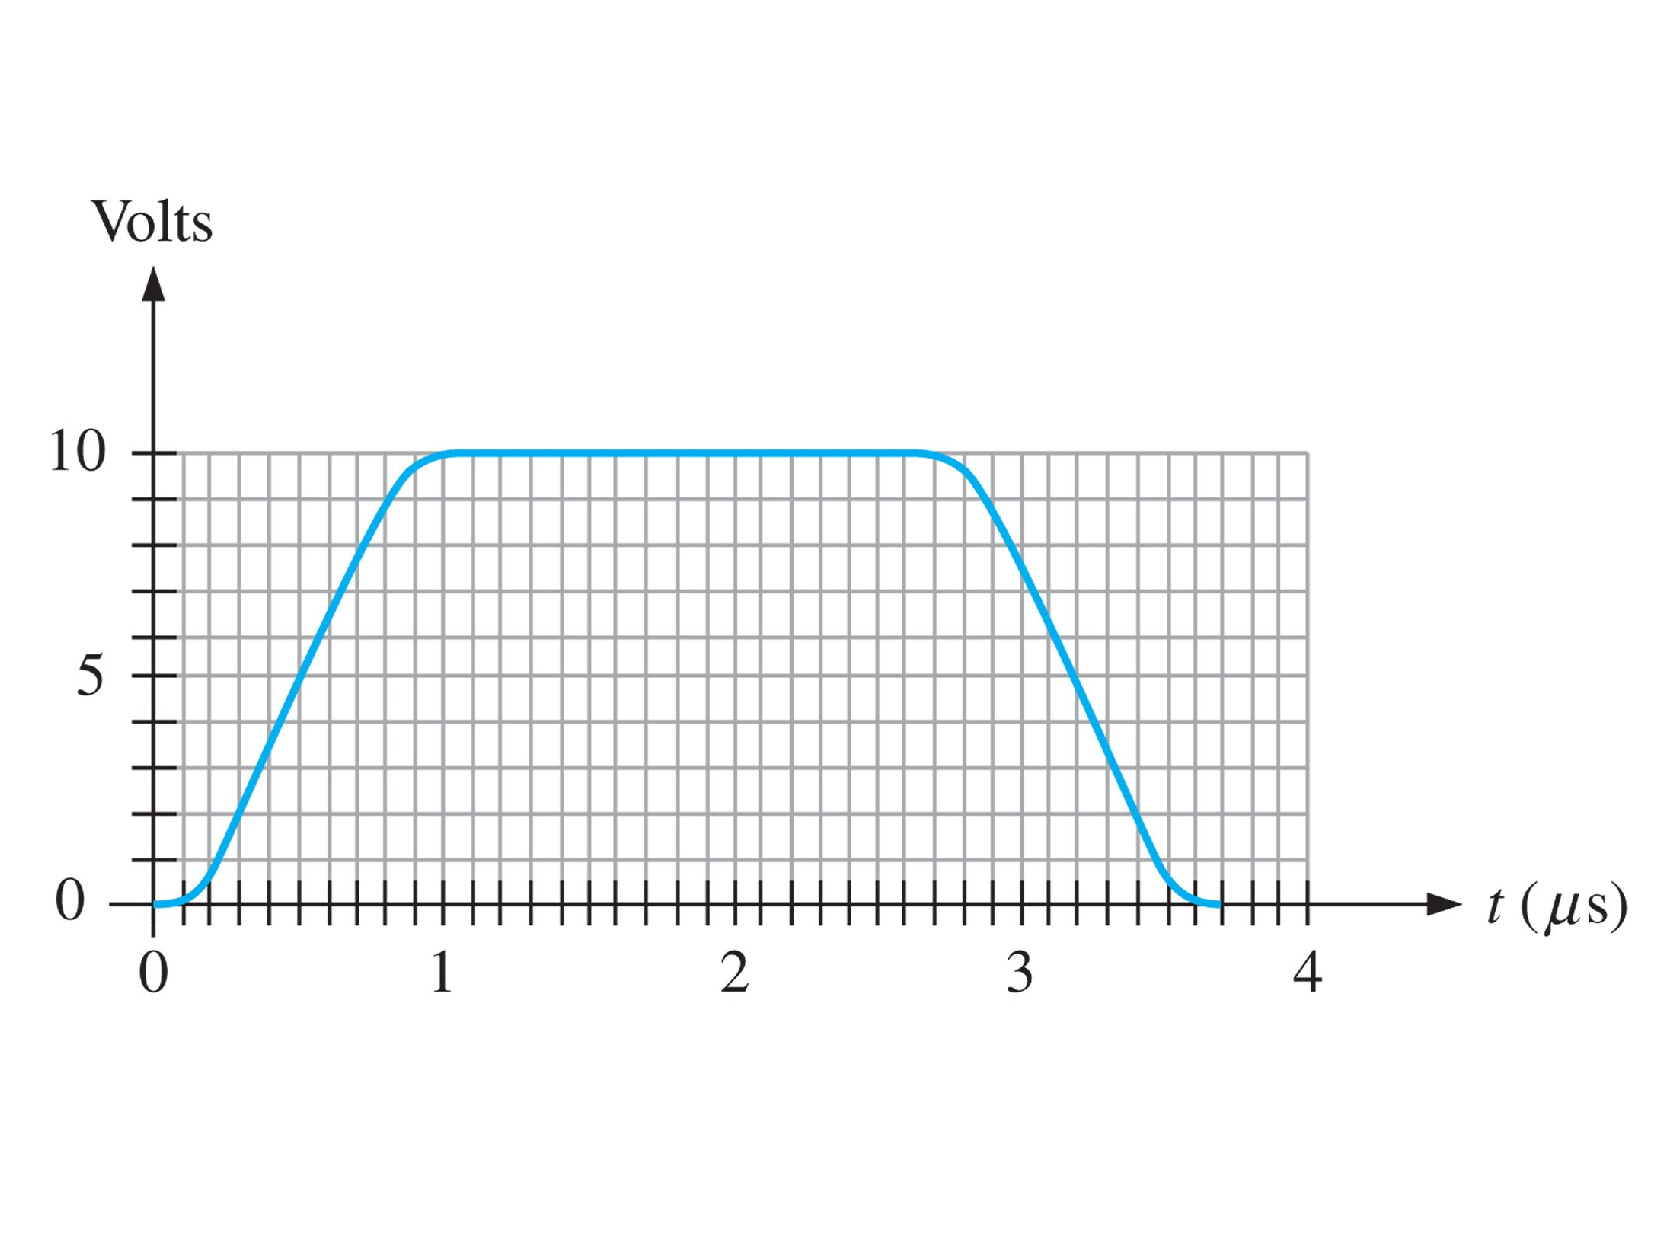
\includegraphics[width=0.3\textwidth,trim=0cm 2cm 0cm 2cm,clip=true]{logicPulse1.pdf}
\caption{\label{fig:logicPulse1} The digital pulse for exercise 7.}
\end{figure}
\item Exercise 8: The period is 4 ms.
\item Exercise 9: The frequency is the inverse of the period, so 0.25 kHz.
\begin{figure}[ht]
\centering
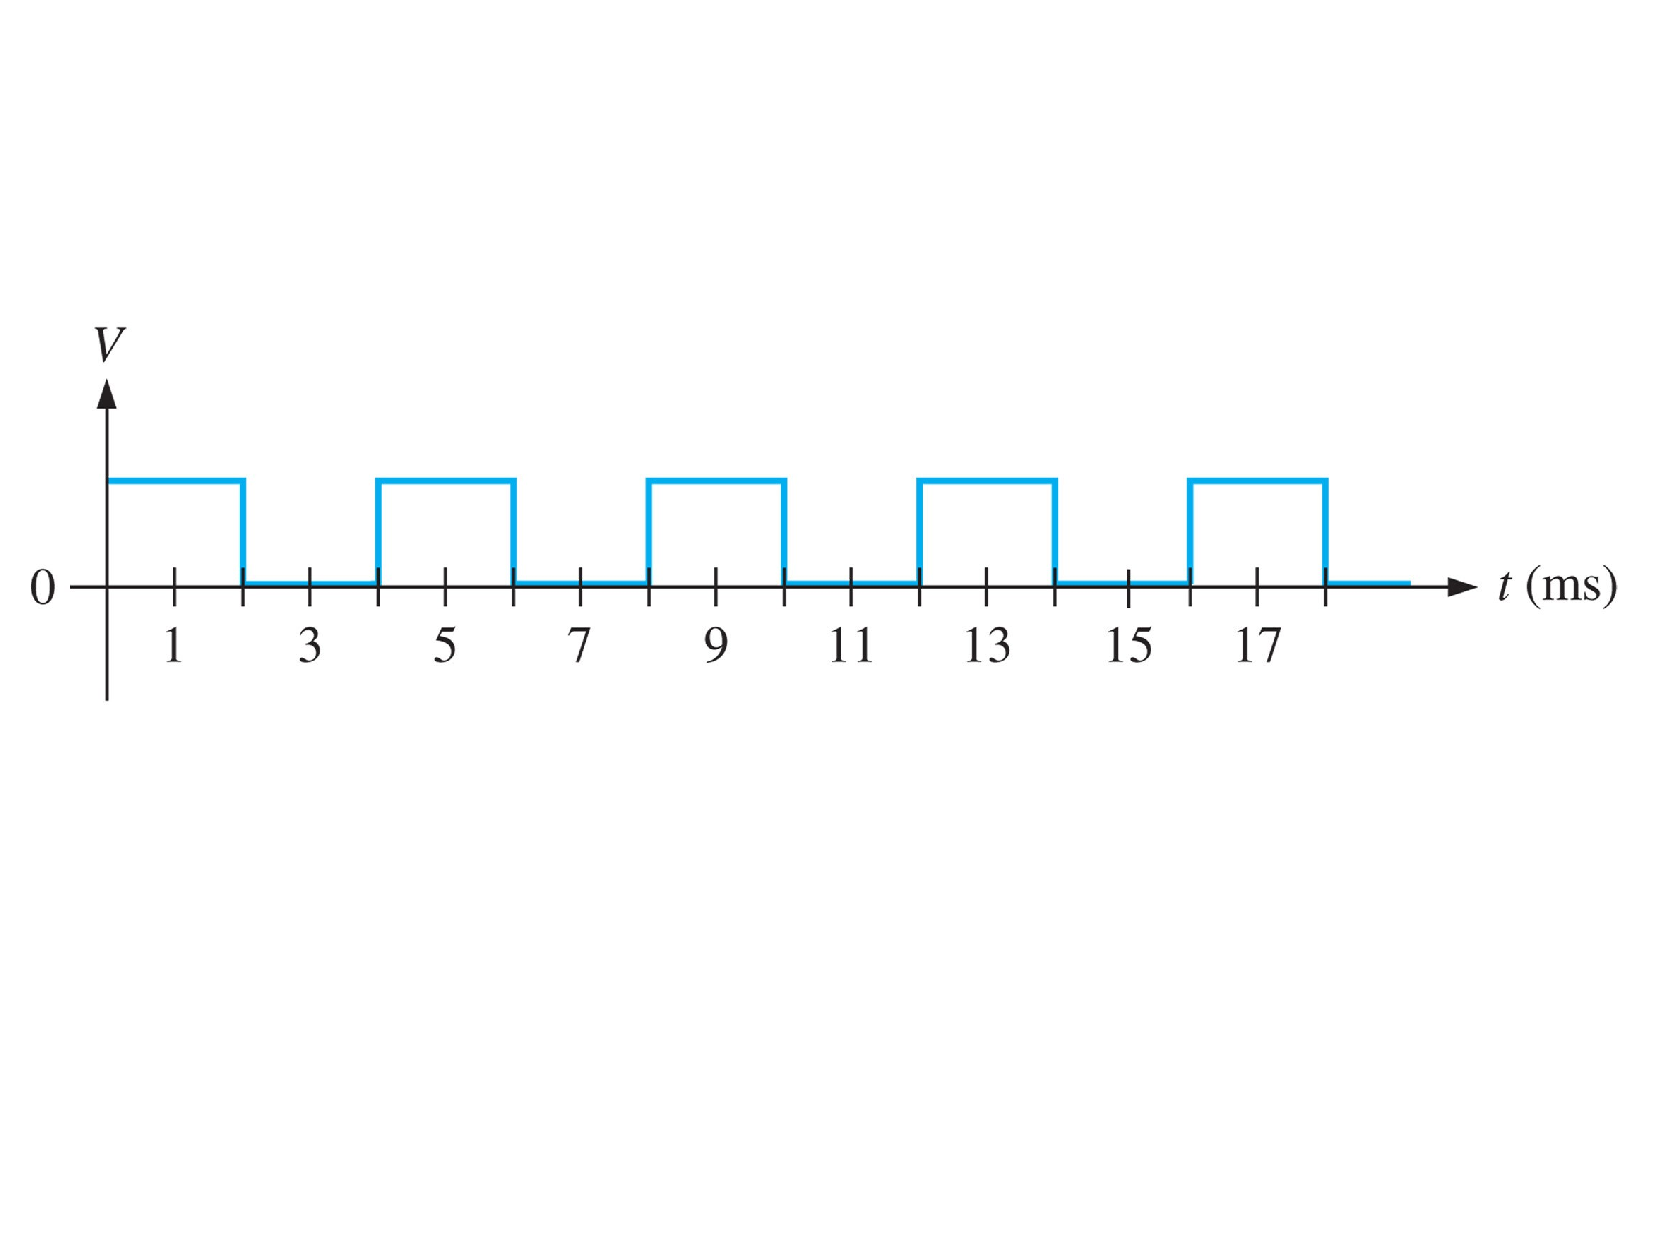
\includegraphics[width=0.4\textwidth,trim=0cm 6cm 0cm 6cm,clip=true]{logicPulse2.pdf}
\caption{\label{fig:logicPulse2} The bitstream/timing diagram for exercise 8.}
\end{figure}
\item Exercise 10: This is an example of a periodic signal.  (\textit{It's a clock signal}).
\item Exercise 10: The duty cycle is 50\%.  The pulse width is 2 ms and the period is 4 ms so the ratio is one-half.
\end{enumerate}

\end{document}
